\documentclass[]{article}
\usepackage{mathtools}
\usepackage[pdftex]{graphicx}	
\usepackage{amsmath,amsfonts,amsthm}	
\usepackage{tikz}
\usetikzlibrary{chains, positioning}
\newtheorem{theorem}{Theorem}[section]
\newtheorem{lemma}[theorem]{Lemma}
\newtheorem{proposition}[theorem]{Proposition}
\newtheorem{corollary}[theorem]{Corollary}
\usepackage{sidecap}
\usepackage{polski}
\usepackage[utf8]{inputenc}
\theoremstyle{definition}
\newtheorem{definition}{Definition}[section]

\usetikzlibrary{calc,arrows}

%opening
\title{Activation functions}
\author{Rafa\l \vspace{1cm} Skrzypiec}
\date{}
\begin{document}
\maketitle

\section{Funkcje aktywacji}

Funckja aktywacji to funkcja, która działa na każdy neuron w sieci neuronowej, jako argument przyjmuje sumę iloczynów wartości neuronów z warstwy poprzedzającej i odpowiadających im wag. Każda z warstw sieci neuronowej może mieć zdefiniowaną inną funckję aktywacji.

Perceptron, który był inspiracją powstania sieci neuronowcyh został skonstruowany jako uproszczony model biologicznego neuronu. W neurobiologii, neuron jest 
komórką, która odbiera, przetwarza i przesyła informacje wykorzystując elektryczne i chemiczne sygnały. Neurony połączone są ze sobą przez synapsy, jeden neuron może otrzymywać informacje od wielu komórek nerwowych. Jeśli suma sygnałów elektrycznych z wejściowych synaps przekroczy pewien próg, wtedy neuron transmituje dalej sygnał elektryczny. Perceptron naśladował ten mechanizm stosując przedstawioną w lewym górnym rogu na Rys.~\ref{fig:activations} funckję Heaviside'a jako funkcję aktywacji. Funkcja przyjmuję wartość jeden jeśli suma wartości wejściowych jest większa od zera, w innym przypadku funkcja przyjmuje wartość zero i neuron nie propaguje sygnału. Perceptron jest najprostszym przykładem sieci neuronowej.

Wyniki badań przeprowadzonych przez [publikacja, publikacja] pokazały, że wśród pożądanych cech funkcji aktywacji znajdują się atrybuty, których funkcja Heaviside'a nie posiada, z tego powodu nie jest w praktyce często stosowana.

Koniecznym wymaganiem jest nieliniowość stosowanej funkcji, jest to cecha, która pozwala sieci neuronowej odwzorować nieliniowe zależności [LeCun, Cybenko?, Hornik]. Jedynym wyjątkiem od reguły jest stosowanie w problemach regresyjnych funkcji tożsamościowej w ostatniej warstwie wyjściowej. Dobrze gdy funkcja posiada ciągłą pochodną, pozwala to na stosowanie metod optymizacji opartych o obliczanie gradientu. Tu wyjątkiem jest stosowana poprawiona jednostka liniowa (ReLU), również przedstawiona na Rys.~\ref{fig:activations}. Zakładając, że w zerze jej gradient równy jest zero możemy skorzystać z jej wielu zalet. Wśród nich wymienia się dokładniejsze odwzorowanie obserwowanego w neurobiologii zjawiska -- tylko neurony, które otrzymały odpowiednio silny sygnał są aktywowane. Brak podatności na przeuczenie, podczas inicjalizacji sieci losowymi wagami, tylko około 50\% ukrytych neuronów jest aktywowanych. Brak problemu znikającego gradientu uniemożliwiającego uczenie, w porównaniu do sigmoidy, u której wysyca się on w obu kierunkach. Jest to również funkcja często wykorzystywana w metodach głębokiego uczenia. W warstwach splotowych sieci która służy do rozpoznawania obrazów wykorzystamy ReLU poszukując atrybutów, które nie zmieniają się podczas jej użycia.
%
\begin{figure}[h!]
	\centering
	\includegraphics[width=\linewidth]{activations14_12}
	\caption{Kilka przykładów często stosowanych funkcji aktywacji.}
	\label{fig:activations}
\end{figure}
%
%
\subsection{Funkcje sigmoidalne}
%
Częstym wyborem funkcji aktywacji są funkcje sigmiodalne. Jest to grupa monotonicznie rosnących funkcji, których zbiór wartości jest ograniczony przez asymptoty o skończonych wartościach, do których wartość funkcji dąży w $\pm \infty$ [lecun98]. Jednym z najczęściej wykorzystywanych przykładów funkcji sigmoidalnych jest sigmoida zdefiniowana równaniem
%
\begin{equation}
\sigma(x) = \frac{1}{1+e^{-x}}.
\end{equation}
%
Sigmoida jest różniczkowalna w każdym punkcie co pozwala używać podczas procesu uczenia metod optymizacji wykorzysujących gradient. Ponadto pochodna względem argumentu $x$ wyraża się prostą relacją
%
\begin{equation}
\frac{d}{dx} \sigma(x)= \sigma(x)\left(1 - \sigma(x)\right).
\end{equation}
%
%
\begin{figure}[h!]
	\centering
	\includegraphics[width=\linewidth]{sigmoid14_8}
	\caption{Przykład funkcji sigmoidalnej - sigmoida, $\sigma(x) = \frac{1}{1+e^{-x}}$}
\end{figure} 

Innym przykładem często wykorzystywanej w sztucznych sieciach neuronowych funkcji sigmoidalnej jest tangens hyperboliczny (prawy dolny róg Rys. \ref{fig:activations}). Wzór tej funkcji możemy wyrazić korzystając z definicji sigmoidy
\begin{equation}
\tanh(x) = 2\sigma(2x)-1
\end{equation}
%
Jedną z zalet tej funkcji jest symetryczność względem początku układu współrzędnych.
%
\subsection{Interpretacja probabilistyczna sigmoidy}
%
Zastosowanie sigmoidy jako funkcji aktywacji naturalnie wynika z postaci prawdopodobieństwa a posteriori w Bayesowskim podejściu do problemu klasyfikacji dwóch klas.
%
Rozważmy sztuczną sieć neuronową z jedną warstwą ukrytą oraz funkcję dyskryminacyjną $y(\mathbf{x})$ taką, że wektor $\mathbf{x}$ jest przypisany do klasy $C_1$ jeśli $y(\mathbf{x}) > 0$ i do klasy $C_2$ jeśli $y(\mathbf{x}) < 0$.
\\
W najprostszej, liniowej formie funkcja może być zapisana jako:
%
\begin{equation}
y(\mathbf{x}) = \mathbf{w}^\mathsf{T} \mathbf{x} + b_0.
\label{sum}
\end{equation}
%
Wektor $\mathbf{w}$, to $d$-wymiarowy wektor wag, natomiast parametr $b_0$ to bias.
%
Rozważmy funkcję $g(\cdot)$ nazywaną dalej funkcją aktywacji, która jako argument przyjmuje jako argument sumę z równania (\ref{sum}):
%
\begin{equation}
y = g\left(\mathbf{w}^\mathsf{T} \mathbf{x} + b_0 \right)
\end{equation}
%
\def\layersep{2.5cm}

	\begin{SCfigure}
		\centering

	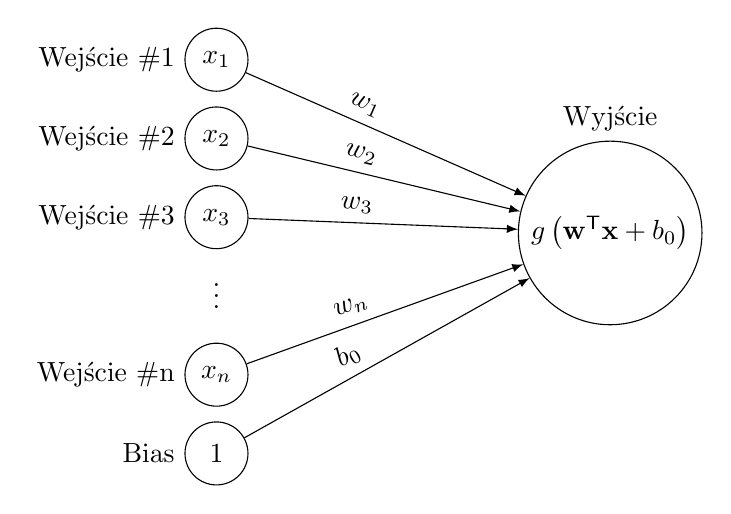
\begin{tikzpicture}
	[   cnode/.style={draw=black,draw=black,fill=#1,minimum width=8mm,circle},
	]
	\tikzset{normal arrow/.style={draw,-latex}}
	\node[cnode=white,label=90:Wyjście] (s) at (5,-3.2) {$ g\left(\mathbf{w}^\mathsf{T} \mathbf{x} + b_0 \right)$};
	\node at (0,-3.9) {$\vdots$};
	
	\node[cnode=white,label=180:Bias] (x-5) at (0,-6) {1};
	
	\foreach \x in {1,...,4}
	{
		\pgfmathparse{\x<4 ? \x : "n"}	   
		\ifnum \x = 4
		\node[cnode=white,label=180:Wejście \#n] (x-\x) at (0,{-1*\x-div(\x,4)}) {$x_{n}$};
		
		\else
		
		\node[cnode=white,label=180:Wejście \#\pgfmathresult] (x-\x) at (0,{-1*\x-div(\x,4)}) {$x_{\x}$};
		\fi
		\path[normal arrow] (x-\x) -- node[above,sloped,pos=0.4] {$w_{\pgfmathresult}$} (s);
	}
	\path[normal arrow] (x-5) -- node[above,sloped,pos=0.4] {$b_0$} (s);	
	\end{tikzpicture}
	\caption{ Reprezentacja funkcji dyskryminacyjnej $y(x)$ w postaci diagramu sieci neuronowej, mającej $n$ wejść, parametr bias i jedno wyjście.  }
	\end{SCfigure}
%
Załóżmy, że funkcja rozkładu prawdopodobieństwa danych pod warunkiem klasy $C_k$ zadane jest przez wielowymiarowy rozkład normalny z równymi macierzami kowariancji $ \Sigma_1 = \Sigma_2 = \Sigma$
%
\begin{equation}
p(x|C_k) = \frac{1}{\left(2 \pi\right)^{\frac{d}{2}} \left| \Sigma \right|^{\frac{1}{2}}} \exp \left[ -\frac{1}{2} \left(\mathbf{x} - \mathbf{\mu}_k\right)^\mathsf{T} \Sigma^{-1} \left(\mathbf{x} - \mathbf{\mu}_k \right) \right].
\end{equation}
%
Prawdopodobieństwo a posteriori klasy $C_1$ można zapisać używając twierdzenia Bayesa:
%
\begin{eqnarray}
	p(C_1 | \mathbf{x}) &=& \frac{p(\mathbf{x}|C_1) p(C_1)}{ p(\mathbf{x}|C_1) p(C_1) + p(\mathbf{x}|C_2)p(C_2)} \nonumber\\
			   &=& \frac{1}{1 + \frac{p(\mathbf{x}|C_2)p(C_2)}{p(\mathbf{x}|C_1)p(C_1)}} \nonumber\\ 
			   &=& \frac{1}{1 + \exp(-a)},
\end{eqnarray}
%
gdzie
%
\begin{eqnarray}
 a &=& \ln \frac{p(\mathbf{x}|C_1)p(C_1)}{p(\mathbf{x}|C_2)p(C_2)} \nonumber \\
 &=& \left( \mu_1 - \mu_2 \right)^{\mathsf{T}} \Sigma^{-1} \mathbf{x}  - \frac{1}{2} \mu_1^\mathsf{T}\mu_1 + \frac{1}{2} \mu_2^\mathsf{T} \Sigma^{-1} \mu_2 + \ln \frac{p(C_1)}{p(C_2)},
\end{eqnarray}
%
pamiętając o tym, że macierz kowariancji jest symetryczna otrzymujemy
%
\begin{subequations}
	\begin{align}
		\mathbf{x} &= \Sigma^{-1} \left(\mu_1 - \mu_2\right)\\
		b_0 &= - \frac{1}{2} \mu_1^\mathsf{T}\mu_1 + \frac{1}{2} \mu_2^\mathsf{T} \Sigma^{-1} \mu_2 + \ln \frac{p(C_1)}{p(C_2)}
	\end{align}
\end{subequations}
%
Zatem widzimy, że użycie funkcji aktywacji w postaci sigmoidy pozwala nie tylko dokonać decyzji klasyfikacji ale również interpretować wynik funkcji dyskryminacyjnej jako prawdopodobieństwa a posteriori.
%
\end{document}



\def\layersep{2.5cm}
\begin{center}
	
	
	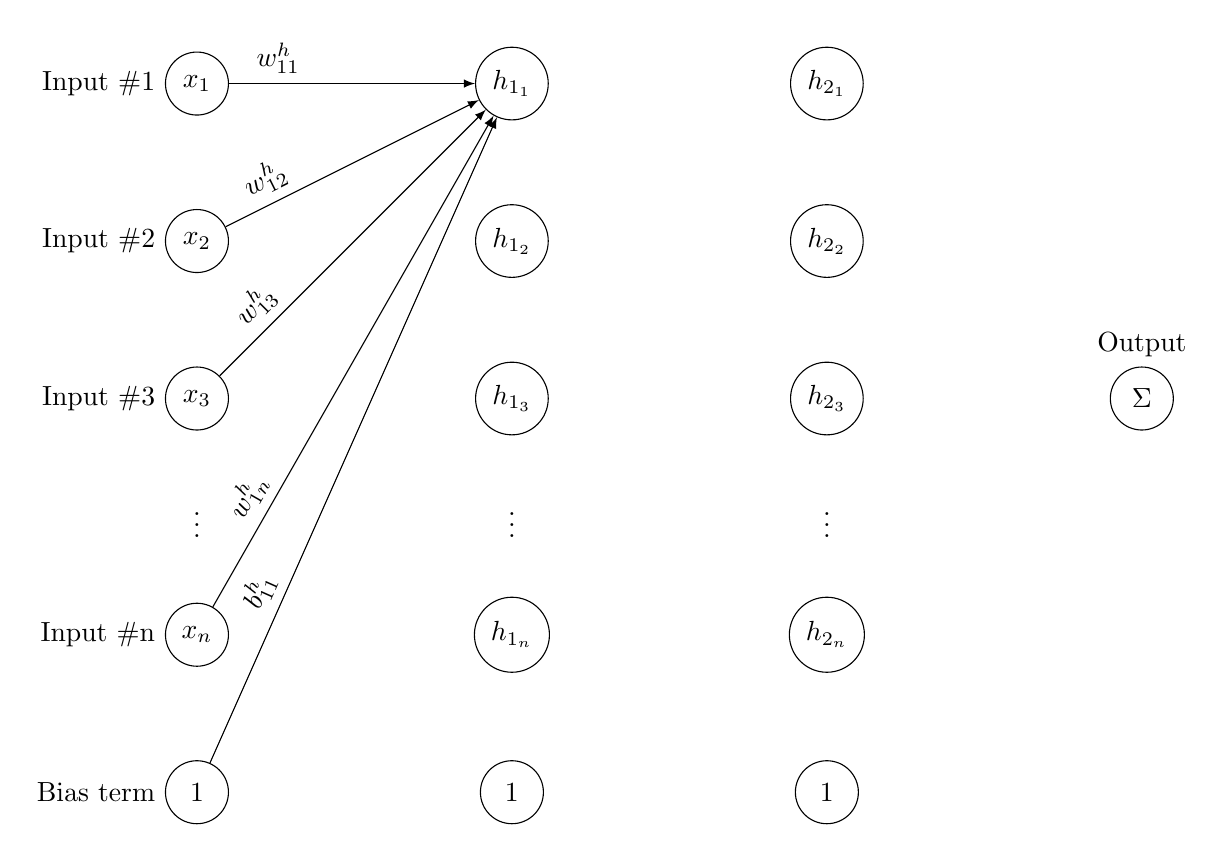
\begin{tikzpicture}
	[   cnode/.style={draw=black,draw=black,fill=#1,minimum width=8mm,circle},
	]
	\tikzset{normal arrow/.style={draw,-latex}}
	\node[cnode=white,label=90:Output] (s) at (12,-6) {$\Sigma$};
	\node at (0,-7.5) {$\vdots$};
	
	\node[cnode=white,label=180:Bias term] (x-5) at (0,-11) {1};
	
	\node at (4,-7.5) {$\vdots$};
	
	\node at (8,-7.5) {$\vdots$};
	
	\node[cnode=white,label=180:] (p-5) at (4,-11) {$1$};
	
	\node[cnode=white,label=180:] (z-5) at (8,-11) {$1$};
	
	
	\foreach \x in {1,...,4}
	{
		\pgfmathparse{\x<4 ? \x : "n"}	   
		\ifnum \x = 4
		\node[cnode=white,label=180:Input \#n] (x-\x) at (0,{-2*\x-div(\x,4)}) {$x_{n}$};
		\node[cnode=white,label=90:] (p-\x) at (4,{-2*\x-div(\x,4)}) {$h_{1_{n}}$};
		
		\node[cnode=white,label=90:] (z-\x) at (8,{-2*\x-div(\x,4)}) {$h_{2_{n}}$};
		
		\else
		
		\node[cnode=white,label=180:Input \#\pgfmathresult] (x-\x) at (0,{-2*\x-div(\x,4)}) {$x_{\x}$};
		\node[cnode=white,label=90:] (p-\x) at (4,{-2*\x-div(\x,4)}) {$h_{1_{\x}}$};
		
		\node[cnode=white,label=90:] (z-\x) at (8,{-2*\x-div(\x,4)}) {$h_{2_{\x}}$};
		
		\fi
	}
	
	
	\foreach \x in {1,...,5}
	{   
		\foreach \y in {1,...,1}
		{   
			\pgfmathparse{\x<4 ? \x : "n"}
			\ifnum \x=1
			\ifnum \y=4
			\path[normal arrow] (x-\x) -- (p-\y) node[above,sloped,pos=0.15] {};
			
			\else
			\path[normal arrow] (x-\x) -- (p-\y) node[above,sloped,pos=0.2] {$w^h_{11}$};
			\fi
			\else
			\ifnum \x=5
			\path[normal arrow] (x-\x) -- (p-\y)node[above,sloped,pos=0.25] {$b^h_{11}$}; 	
			\else
			\path[normal arrow] (x-\x) -- (p-\y)node[above,sloped,pos=0.2] {$w^h_{1\pgfmathresult}$}; 	
			\fi
			\fi
			
			
			
			
			
			
			%\draw (x-\x) -- (p-\y) node[above,sloped,pos=0.3] {$\omega_{\x\y}$};
		}
		
		
	}
	\end{tikzpicture}
	
\end{center}